\chapter{Neural Stochastic Flows}
\label{chap:nsf}

The reconstruction of a gappy light curve was framed in \S\,\ref{ssec:RebMap} as an ill-posed problem, best approached by returning a distribution of signals consistent with the data rather than a single curve. The damped random walk introduced in Chapter \ref{chap:simulation} already provides such a probabilistic description because it is a Gaussian process and the transition between any two epochs has a known analytic form. The method adopted in this thesis replaces that transition with a flexible one learned directly from data, using neural stochastic flows (NSF; \cite{Kiyohara2025SNF}). The motivation is twofold, flexibility and efficiency. A learned transition can in principle capture departures from the damped random walk that a fixed kernel cannot, and, more generally, neural stochastic flows are \textit{solver-free}: they model the transition density of a stochastic differential equation directly, without the numerical integration that conventional neural SDEs require. In the damped random walk case considered here the transition is analytically known, which provides an exact reference against which the learned model can be validated (see Chapter \ref{chap:reconstruction}). 

\section{Normalizing Flows}
\label{sec:normflows}

A \textit{normalizing flow} (NF) transforms a simple probability distribution, typically a standard normal $z \sim p_Z(z)$, into a more complex one through a sequence of invertible and differentiable mappings \parencites{Rezende2016VIwNF}{Kobyzev2021NFRev}. A sample is generated by passing the base variable through the map, $y = g_\theta(z)$, the \textit{generative direction}. Because the map is invertible, one can also go back from $y$ to $z$ through $z = f_\theta(y) = g_\theta^{-1}(y)$, the \textit{normalizing direction}, and the density of $y$ follows from the change-of-variables formula,
\begin{equation}
    \label{eq:changeofvars}
    p_Y(y) = p_Z\big(f_\theta(y)\big)\,\big|\det J_{f_\theta}(y)\big|,
\end{equation}
where $J_{f_\theta}$ is the Jacobian of the inverse map. The base density $p_Z$ is known and the Jacobian term, the \textit{volume correction}, accounts for the change of volume induced by the transformation, so Eq. \ref{eq:changeofvars} yields an exact density for $y$ (Figure \ref{fig:changeofvars}). This exactness, together with the ability both to sample and to evaluate densities, is what makes normalizing flows well suited to modelling complex distributions, and it means the model can be trained simply by maximising the likelihood of the data under Eq. \ref{eq:changeofvars} \parencite{Kobyzev2021NFRev}.

\begin{figure}[t]
    \centering
    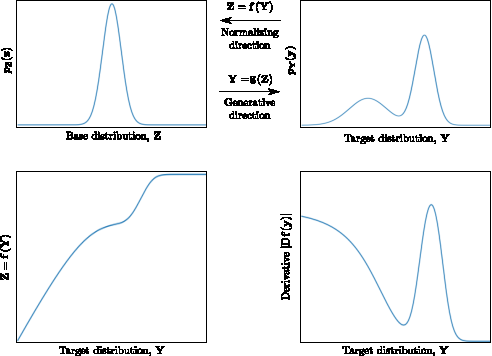
\includegraphics[width=0.82\textwidth]{assets/4_figures/NFSimple.pdf}
    \caption[The change of variables underlying a normalizing flow]{\label{fig:changeofvars} The change of variables of Eq. \ref{eq:changeofvars}. Top left: the base density $p_Z$. Top right: the target density $p_Y$. A bijective map $g$ transforms one into the other, with inverse $f$. Bottom left: the inverse map $f$. Bottom right: its absolute Jacobian, which rescales the density so that probability is conserved. Adapted from \cite{Kobyzev2021NFRev}.}
\end{figure}

For Eq. \ref{eq:changeofvars} to be practical, the transformation must satisfy two requirements: it must be easily invertible, and its Jacobian determinant must be cheap to compute \parencite{Kobyzev2021NFRev}. A construction that meets both, and the one on which the model used here is built, is the \textit{coupling flow} \parencite{Dihn2015Coupling}. The input is split into two partitions; one is left unchanged, and the other is transformed by a bijection whose parameters are produced by a \textit{conditioner} network taking the unchanged partition as input,
\begin{equation}
    \label{eq:coupling}
    y_\mathrm{A} = x_\mathrm{A}, \qquad y_\mathrm{B} = x_\mathrm{B} \odot \exp\!\big(s(x_\mathrm{A})\big) + t(x_\mathrm{A}),
\end{equation}
where $s$ and $t$ are the scale and shift functions and $\odot$ is the elementwise product. This is the affine coupling layer of RealNVP \parencite{Dinh2017RealNVP}. It is trivially inverted, since the unchanged partition $x_\mathrm{A} = y_\mathrm{A}$ recovers the arguments of $s$ and $t$, and its Jacobian is triangular, so its determinant is simply the product of the diagonal, $\prod_j \exp(s(x_\mathrm{A}))_j$. Because neither the inverse nor the determinant requires inverting or differentiating $s$ and $t$, these functions can be arbitrarily complex neural networks. A single such layer leaves one partition untouched, so the partitions are alternated between successive layers, and stacking many layers yields an expressive invertible map.

\section{From Static Densities to Transition Laws}
\label{sec:nsf}

Neural stochastic flows extend this construction from a single \textit{static} density to the \textit{transition law} of a stochastic process \parencite{Kiyohara2025SNF}. Rather than modelling one distribution $p_Y(y)$, they model the conditional distribution of a future state given a current state and an elapsed time,
\begin{equation}
    \label{eq:transition}
    p_\theta\big(x_t \mid x_s, \Delta t\big),
    \qquad \Delta t = t - s,
\end{equation}
that is, the distribution of the state $x_t$ at time $t$ given that the process was at $x_s$ at the earlier time $s$. This conditional is defined in the same way as an ordinary flow, but with the transformation now conditioned on the starting state and the elapsed time: a Gaussian noise variable $\epsilon \sim \mathcal{N}(0, I)$ is passed through a conditional normalizing flow,
\begin{equation}
    \label{eq:flowmap}
    x_t = F_\theta\big(x_s, \Delta t, \epsilon\big).
\end{equation}
For fixed $x_s$ and $\Delta t$, different draws of $\epsilon$ produce different possible future states $x_t$, and together they define the conditional density $p_\theta(x_t \mid x_s, \Delta t)$ of Eq. \ref{eq:transition}. Modelling this density directly, rather than the individual paths of the process, is what allows a state at any elapsed time to be sampled in a single step, without iterative integration (Figure \ref{fig:nsfsolutions}).

\begin{figure}[t]
    \centering
    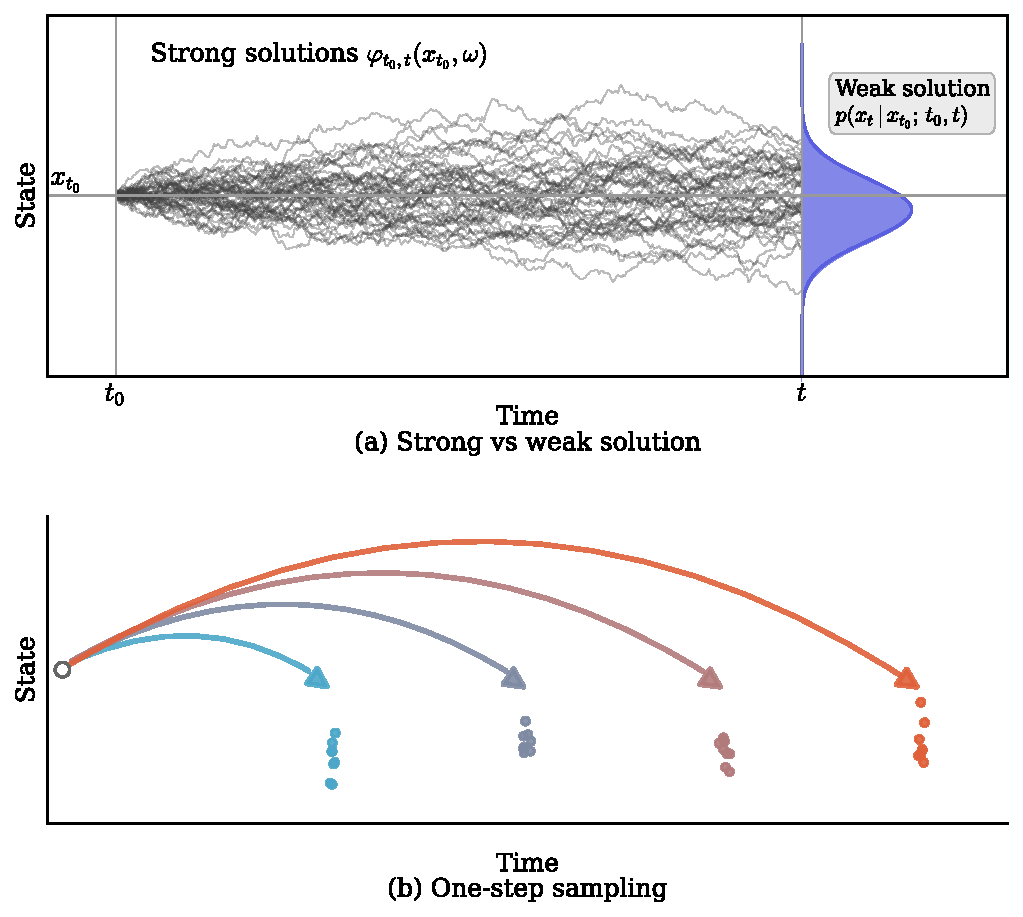
\includegraphics[width=0.78\textwidth]{assets/4_figures/nsf_solutions.pdf}
    \caption[Strong and weak solutions of an SDE and one-step sampling]{\label{fig:nsfsolutions} (a) The \textit{strong solution} of a stochastic differential equation is an ensemble of paths $\varphi_{t_0,t}(x_{t_0}, \omega)$ diverging from a common initial state; the \textit{weak solution} is the transition density $p(x_t \mid x_{t_0}; t_0, t)$ they define at a later time, shown at the right edge. Neural stochastic flows model this density directly. (b) Because the density is modelled directly, samples at any elapsed time can be drawn in a single step, without the iterative integration that path-based methods require. Adapted from \cite{Kiyohara2025SNF}.}
\end{figure}

Concretely, the sample is drawn by first initializing a state-dependent Gaussian that mirrors an Euler-Maruyama step, with a mean displaced from $x_s$ by a drift scaled by $\Delta t$ and a variance scaled by $\sqrt{\Delta t}$,
\begin{equation}
    \label{eq:base}
    z = \underbrace{x_s + \Delta t\,\mathrm{MLP}_\mu(c)}_{\mu(c)} + \underbrace{\sqrt{\Delta t}\,\mathrm{MLP}_\sigma(c)}_{\sigma(c)} \odot\, \epsilon, \qquad c := (x_s, \Delta t),
\end{equation}
and then passing it through a sequence of coupling layers of the form of Eq. \ref{eq:coupling}, whose scale and shift functions are now additionally conditioned on $c$ and multiplied by $\Delta t$. The map $F_\theta$ is constrained in this way so that the transition density inherits the defining properties of the solution of a stochastic differential equation \parencite{Kiyohara2025SNF}. Two are relevant here. The \textit{identity} property requires that a zero time gap returns the input state, $p_\theta(x_t \mid x_s, 0) = \delta(x_t - x_s)$; the explicit factors of $\Delta t$ in Equations \ref{eq:base} and \ref{eq:coupling} enforce this, since both the Gaussian and every coupling layer collapse to the identity as $\Delta t \to 0$. The \textit{stationarity} property requires that, for a time-homogeneous process, the transition depend only on the gap $\Delta t$ and not on absolute time; since the damped random walk is autonomous, the conditioner omits absolute time and depends on $\Delta t$ alone. A third property, discussed in the following section, ties transitions of different lengths together.

This learned transition plays the role of the damped random walk step in place of the analytic transition of the Ornstein-Uhlenbeck process (Chapter \ref{chap:simulation}), the flexible map $F_\theta$ models the variability between any two epochs, while reducing to the correct transition when the data are generated by a damped random walk.

\section{Triplets and Stochastic Bridges}
\label{sec:bridges}

Reconstructing a gap requires the distribution of a state that lies \textit{between} two observations, not merely one that follows from a single earlier state. This intermediate conditional is modelled by a \textit{stochastic bridge}. Following the training strategy of \textcite{Kiyohara2025SNF}, from each light curve one randomly samples triplets of times $(t_i, t_j, t_k)$ with $t_i < t_j < t_k$, and two models are trained jointly on them. The \textit{flow} model learns the transitions between states, both the direct endpoint transition $p_\theta(x_k \mid x_i, \Delta t_{ik})$ and the two one-step transitions $p_\theta(x_j \mid x_i, \Delta t_{ij})$ and $p_\theta(x_k \mid x_j, \Delta t_{jk})$. The \textit{bridge} model learns the intermediate conditional\footnote{The bridge is denoted $b_\xi$ in the original formulation of \textcite{Kiyohara2025SNF}; it is written $q_\xi$ here to emphasize its role as an auxiliary variational distribution and for consistency with the notation used throughout this work.}
\begin{equation}
    \label{eq:bridge}
    q_\xi\big(x_j \mid x_i, x_k, t_i, t_j, t_k\big),
\end{equation}
the distribution of the middle state given both surrounding states and their times. It is this bridge, conditioned on the two bracketing observations, that performs the gap filling at inference.

The two models are tied together by the third inherited property, the \textit{flow property}, which requires that the transition density satisfy the Chapman-Kolmogorov relation: the direct transition from $x_i$ to $x_k$ must equal the composition of the two one-step transitions through any intermediate state,
\begin{equation}
    \label{eq:chapmankolmogorov}
    p_\theta\big(x_k \mid x_i, \Delta t_{ik}\big) = \int p_\theta\big(x_k \mid x_j, \Delta t_{jk}\big)\, p_\theta\big(x_j \mid x_i, \Delta t_{ij}\big)\,\mathrm{d}x_j.
\end{equation}
Equivalently, the joint distribution of the pair $(x_j, x_k)$ given $x_i$ can be factorized either as a one-step flow from $x_i$ to $x_k$ followed by the bridge that places $x_j$ between them, or as a two-step flow $x_i \rightarrow x_j \rightarrow x_k$; both describe the same distribution and must agree. Enforcing this relation is what forces the flow and the bridge to represent a single, self-consistent stochastic process rather than two unrelated conditionals.

The two sides of Eq. \ref{eq:chapmankolmogorov} cannot be compared directly, since the two-step side requires marginalizing over the intermediate state $x_j$. The bridge $q_\xi$ is therefore introduced as an auxiliary variational distribution, which makes the comparison tractable through variational upper bounds on the Kullback-Leibler divergence between the one-step and two-step transitions, taken in both directions since the divergence is asymmetric. The forward bound, from the one-step to the two-step transition, is
\begin{equation}
    \label{eq:flow12}
    \mathcal{L}_\mathrm{1\text{-}to\text{-}2} = \mathbb{E}\!\left[\log \frac{p_\theta(x_k \mid x_i)\, q_\xi(x_j \mid x_i, x_k)}{p_\theta(x_k \mid x_j)\, p_\theta(x_j \mid x_i)}\right],
\end{equation}
with the expectation over $p_\theta(x_k \mid x_i)\,q_\xi(x_j \mid x_i, x_k)$, and the reverse bound is
\begin{equation}
    \label{eq:flow21}
    \mathcal{L}_\mathrm{2\text{-}to\text{-}1} = \mathbb{E}\!\left[\log \frac{p_\theta(x_j \mid x_i)\, p_\theta(x_k \mid x_j)}{q_\xi(x_j \mid x_i, x_k)\, p_\theta(x_k \mid x_i)}\right],
\end{equation}
with the expectation over $p_\theta(x_j \mid x_i)\,p_\theta(x_k \mid x_j)$. Their sum is the flow-consistency loss, $\mathcal{L}_\mathrm{flow} = \mathcal{L}_\mathrm{1\text{-}to\text{-}2} + \mathcal{L}_\mathrm{2\text{-}to\text{-}1}$. The explicit form of these bounds, as a difference of log-densities evaluated on Monte Carlo samples for a single triplet, is given in Appendix \ref{app:loss}, together with the architecture of the bridge model.

\section{Training Objective}
\label{sec:objective}

The model is trained by minimising a loss with two terms \parencite{Kiyohara2025SNF},
\begin{equation}
    \label{eq:loss}
    \mathcal{L}(\theta, \xi) = \mathcal{L}_\mathrm{data}(\theta) + \lambda\,\mathcal{L}_\mathrm{flow}(\theta, \xi),
\end{equation}
where $\mathcal{L}_\mathrm{data}$ is the negative log-likelihood of the observed transitions under the flow, evaluated through the change-of-variables formula of Eq. \ref{eq:changeofvars}, and $\mathcal{L}_\mathrm{flow}$ is the flow-consistency term of Equations \ref{eq:flow12} and \ref{eq:flow21}, weighted by a hyperparameter $\lambda$. The data term anchors the model to the observed light curves, while the consistency term enforces that the learned transitions compose correctly across time. Both terms are necessary: the consistency term alone admits self-consistent but arbitrary transitions, and it is the data likelihood that ties the learned process to the damped random walk actually present in the light curves. The balance between the two terms is set by $\lambda$, but the results are insensitive to its precise value: varying $\lambda$ over more than an order of magnitude, from $0.03$ to $1.0$, changes the coverage on the low-noise validation set by at most a few per cent, from $0.62$ to $0.60$, and leaves the RMSE unchanged at $0.18$. A value of $\lambda = 0.1$ is used throughout.

\section{Reconstruction}
\label{sec:reconstruction}

Once trained, the bridge performs the gap filling. Reconstructing a gap means conditioning on the observations at \textit{both} of its ends, which is precisely what the bridge does. %Conditioning on the preceding observation alone would be forecasting, not interpolation. T
he flux is reconstructed on a dense grid between each pair of consecutive observations. For a grid point lying between two observations, the bracketing observations provide the conditioning states $x_i$ and $x_k$ and their times, and the bridge $q_\xi$ of Eq. \ref{eq:bridge} gives the distribution of the flux at the intermediate time. Because this distribution can be sampled in a single pass, a set of Monte Carlo realizations of the reconstruction is drawn by sampling the bridge independently at each grid point, as illustrated in Figure \ref{fig:mcsamples}. The reconstruction is summarized by the pointwise median of these samples, taken as the central estimate, and by the interval between the $16$th and $84$th percentiles, which gives the central $68\%$ predictive band. At the observations themselves the reconstruction is pinned to the measured values, so the band closes to zero width there and widens across the interior of an interval, where the elapsed time to the nearest observation is longer and the transition is correspondingly more uncertain. It is this predictive distribution, rather than any single reconstructed curve, that the evaluation of Chapter \ref{chap:reconstruction} assesses.

\begin{figure}[H]
    \centering
    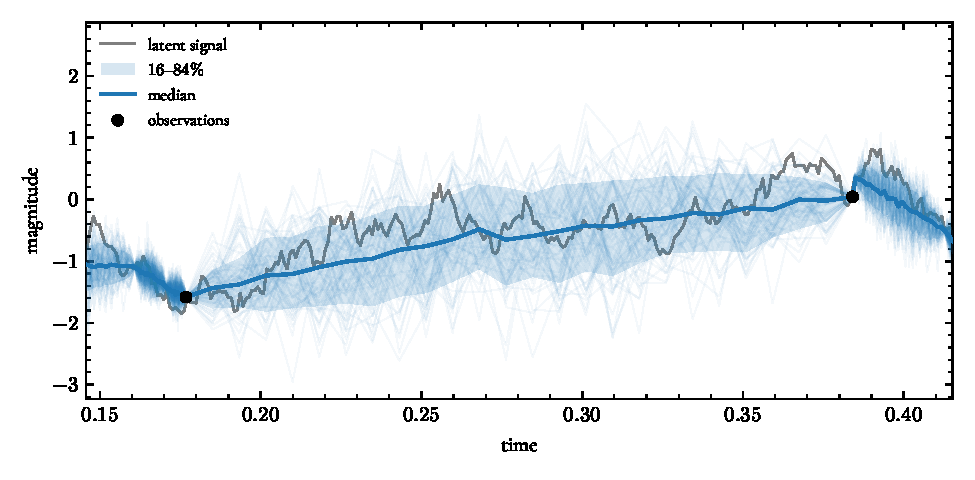
\includegraphics[width=\textwidth]{assets/5_figures/VaryTauExp/MCSamples.pdf}
    \caption[Monte Carlo bridge reconstructions across a gap]{\label{fig:mcsamples} Monte Carlo reconstructions of a single gap in a varying-timescale validation curve. Each thin line is one sample drawn from the bridge conditioned on the two bracketing observations (black); their pointwise median (blue) and central $68\%$ interval (shaded) summarize the ensemble. The samples fan out across the interior of the gap and converge at the endpoints, and together they bracket the latent signal (grey).}
\end{figure}

The flow and bridge are conditioned on the flux values and times alone: the per-epoch measurement uncertainties enter neither their conditioning, nor the training objective, nor the sampling at inference. The predictive intervals of the reconstruction therefore express the variance of the learned process and carry no information about the measurement error of the observations on which they are conditioned. The Gaussian process baseline, by contrast, includes the per-epoch uncertainties directly in its covariance, and it is this difference that underlies the comparison of their calibration in Chapter \ref{chap:reconstruction}.


\section{Implementation}
\label{sec:implementation}

The model is implemented in \textsc{jax} \parencite{JAX2018Github}, building on the publicly available \texttt{jax\_nsf} codebase accompanying \textcite{Kiyohara2025SNF}, from which the flow and bridge architectures and the core training machinery are taken. The change-of-variables likelihood of Eq. \ref{eq:changeofvars} and the variational bounds of Equations \ref{eq:flow12} and \ref{eq:flow21} are differentiated automatically, so the gradients of the loss are obtained straighforward, and the full training step is compiled once and reused across iterations, which makes the repeated evaluation of the loss over many triplets efficient. The flow and bridge are represented as \texttt{equinox} modules \parencite{Kidger2021Equinox}, and only their floating-point array leaves are treated as trainable parameters, with the remaining static structure held fixed during optimisation.

Training minimizes the objective of Eq. \ref{eq:loss} using the Adam optimizer \parencite{Kingma2017Adam} as implemented in \texttt{optax} \parencite{Deepmind2020Optax}, with a learning rate of $2\times10^{-3}$. At each step a batch of sixteen light curves is drawn, and from each a set of thirty-two triplets $(t_i, t_j, t_k)$ is sampled, with the intermediate times drawn log-uniformly so that both short and long gaps are represented. The loss is averaged over the batch and its gradient taken through the compiled step. The zero-padding introduced when the ragged light curves are stored as fixed-size arrays (Chapter \ref{chap:simulation}) is excluded from the loss through a mask, so that only genuine observations contribute.

The simulation of the light curves and the training of the model are carried out in two separate environments. The simulator relies on \texttt{EzTao} \parencite{Yu2022Extao}, whose dependencies conflict with those of \texttt{jax\_nsf}, so the two cannot share an environment. The simulated light curves are written to disk and read back for training, with the saved dataset acting as the only interface between the two stages. This separation keeps the generation of the training set reproducible and independent of the model, so a dataset can be regenerated or reused without retraining.

The contributions of this thesis are in the surrounding framework rather than in the flow architecture itself: the simulation of damped random walk light curves with physically motivated parameters (Chapter \ref{chap:simulation}), the construction of a training set matched to the sampling and noise of a real survey (Chapter \ref{chap:reconstruction}), and the evaluation of the learned model against the analytic transition and a Gaussian process baseline.% The training objective retains both terms of Eq. \ref{eq:loss}, the data-likelihood term being essential for the model to recover the underlying dynamics, point examined in Chapter \ref{chap:reconstruction}.